\documentclass[a4paper,oneside,12pt]{extreport}

\usepackage{mmap}
\usepackage[T2A]{fontenc}
\usepackage[utf8]{inputenc}
\usepackage[english,russian]{babel}

\usepackage[left=30mm, right=15mm, top=20mm, bottom=20mm]{geometry}

\setlength{\parindent}{1.25cm} % Абзацный отступ

\usepackage{setspace}
\onehalfspacing % Полуторный интервал

\frenchspacing % Равномерные пробелы
\usepackage{indentfirst} % Красная строка

\usepackage{microtype}
\sloppy

\usepackage{titlesec}
\titlespacing*{\chapter}{0pt}{-30pt}{8pt}
\titlespacing*{\section}{\parindent}{*4}{*4}
\titlespacing*{\subsection}{\parindent}{*4}{*4}
\titleformat{\chapter}{\LARGE\bfseries}{\thechapter}{20pt}{\LARGE\bfseries}
\titleformat{\section}{\Large\bfseries}{\thesection}{40pt}{\Large\bfseries}

\usepackage{graphicx}
\usepackage{caption}

\usepackage[unicode,pdftex]{hyperref}
\hypersetup{hidelinks}

\usepackage{amsmath}

%% title begin
\usepackage{wrapfig}

\makeatletter
	\def\vhrulefill#1{\leavevmode\leaders\hrule\@height#1\hfill \kern\z@}
\makeatother
%% title end

%% begin code
\usepackage{listings}
\usepackage{xcolor}

\lstset{
	basicstyle=\footnotesize\ttfamily,
	breakatwhitespace=true,
	breaklines=true,
	commentstyle=\color{gray},
	frame=single,
	keywordstyle=\color{blue},
	stringstyle=\color{red},
	tabsize=8
}

\newcommand{\code}[1]{\texttt{#1}}
%% end code


\begin{document}

\begin{titlepage}
	{\large % 14pt instead of 12pt
	\onehalfspacing
	\centering

	\begin{wrapfigure}[7]{l}{0.14\linewidth}
		\vspace{3mm}
		\hspace{-10mm}
		
\includegraphics[width=0.93\linewidth]{inc/img/bmstu-logo}
	\end{wrapfigure}
	{\singlespacing \footnotesize \bfseries Министерство науки и высшего образования Российской Федерации\\Федеральное государственное бюджетное образовательное учреждение\\высшего образования\\<<Московский государственный технический университет\\имени Н.~Э.~Баумана\\ (национальный исследовательский университет)>>\\(МГТУ им. Н.~Э.~Баумана)\\}

	\vspace{-2.2mm}
	\vhrulefill{0.9mm}\\
	\vspace{-7.5mm}
	\vhrulefill{0.2mm}\\
	\vspace{2mm}

	{\doublespacing \small \raggedright ФАКУЛЬТЕТ \hspace{37mm} «Информатика и системы управления»\\
	КАФЕДРА \hspace{17mm} «Программное обеспечение ЭВМ и информационные технологии»\\}

	\vspace{30mm}

	\textbf{ОТЧЁТ}\\
	По лабораторной работе № 2\\
	По курсу: «Моделирование»\\
	Тема: «Распределение случайных величин»\\
	Вариант: 6 $\equiv$ 2 (mod 4)\\

	\vspace{40mm}

	\begin{flushleft}
		\begin{tabular}{lr}
			\textbf{Студент:}        & Керимов~А.~Ш. \\
			\textbf{Группа:}         & ИУ7-74Б       \\
			\textbf{Оценка (баллы):} & \hrulefill    \\
			\textbf{Преподаватель:}  & Рудаков~И.~В. \\
		\end{tabular}
	\end{flushleft}

	\vfill

	Москва\\
	\the\year\\}
\end{titlepage}

\setcounter{page}{2}


\tableofcontents

\chapter{Формализация}

\section{Задание}

В информационный центр приходят клиенты через интервал времени $10 \pm 2$ минуты.
Если все три имеющихся оператора заняты, клиенту отказывают в обслуживании.
Операторы имеют разную производительность и могут обеспечивать обслуживание среднего запроса пользователя за $20 \pm 5$; $40 \pm 10$; $40 \pm 20$.
Клиенты стремятся занять свободного оператора с максимальной производительностью. Полученные запросы сдаются в накопитель.
Откуда выбираются на обработку.
На первый компьютер запросы от 1 и 2-ого операторов, на второй – запросы от 3-его. Время обработки запросов первым и 2-м компьютером равны соответственно 15 и 30 мин. Промоделировать процесс обработки 300 запросов.

\section{Концептульная модель}

\begin{figure}[H]
	\centering
	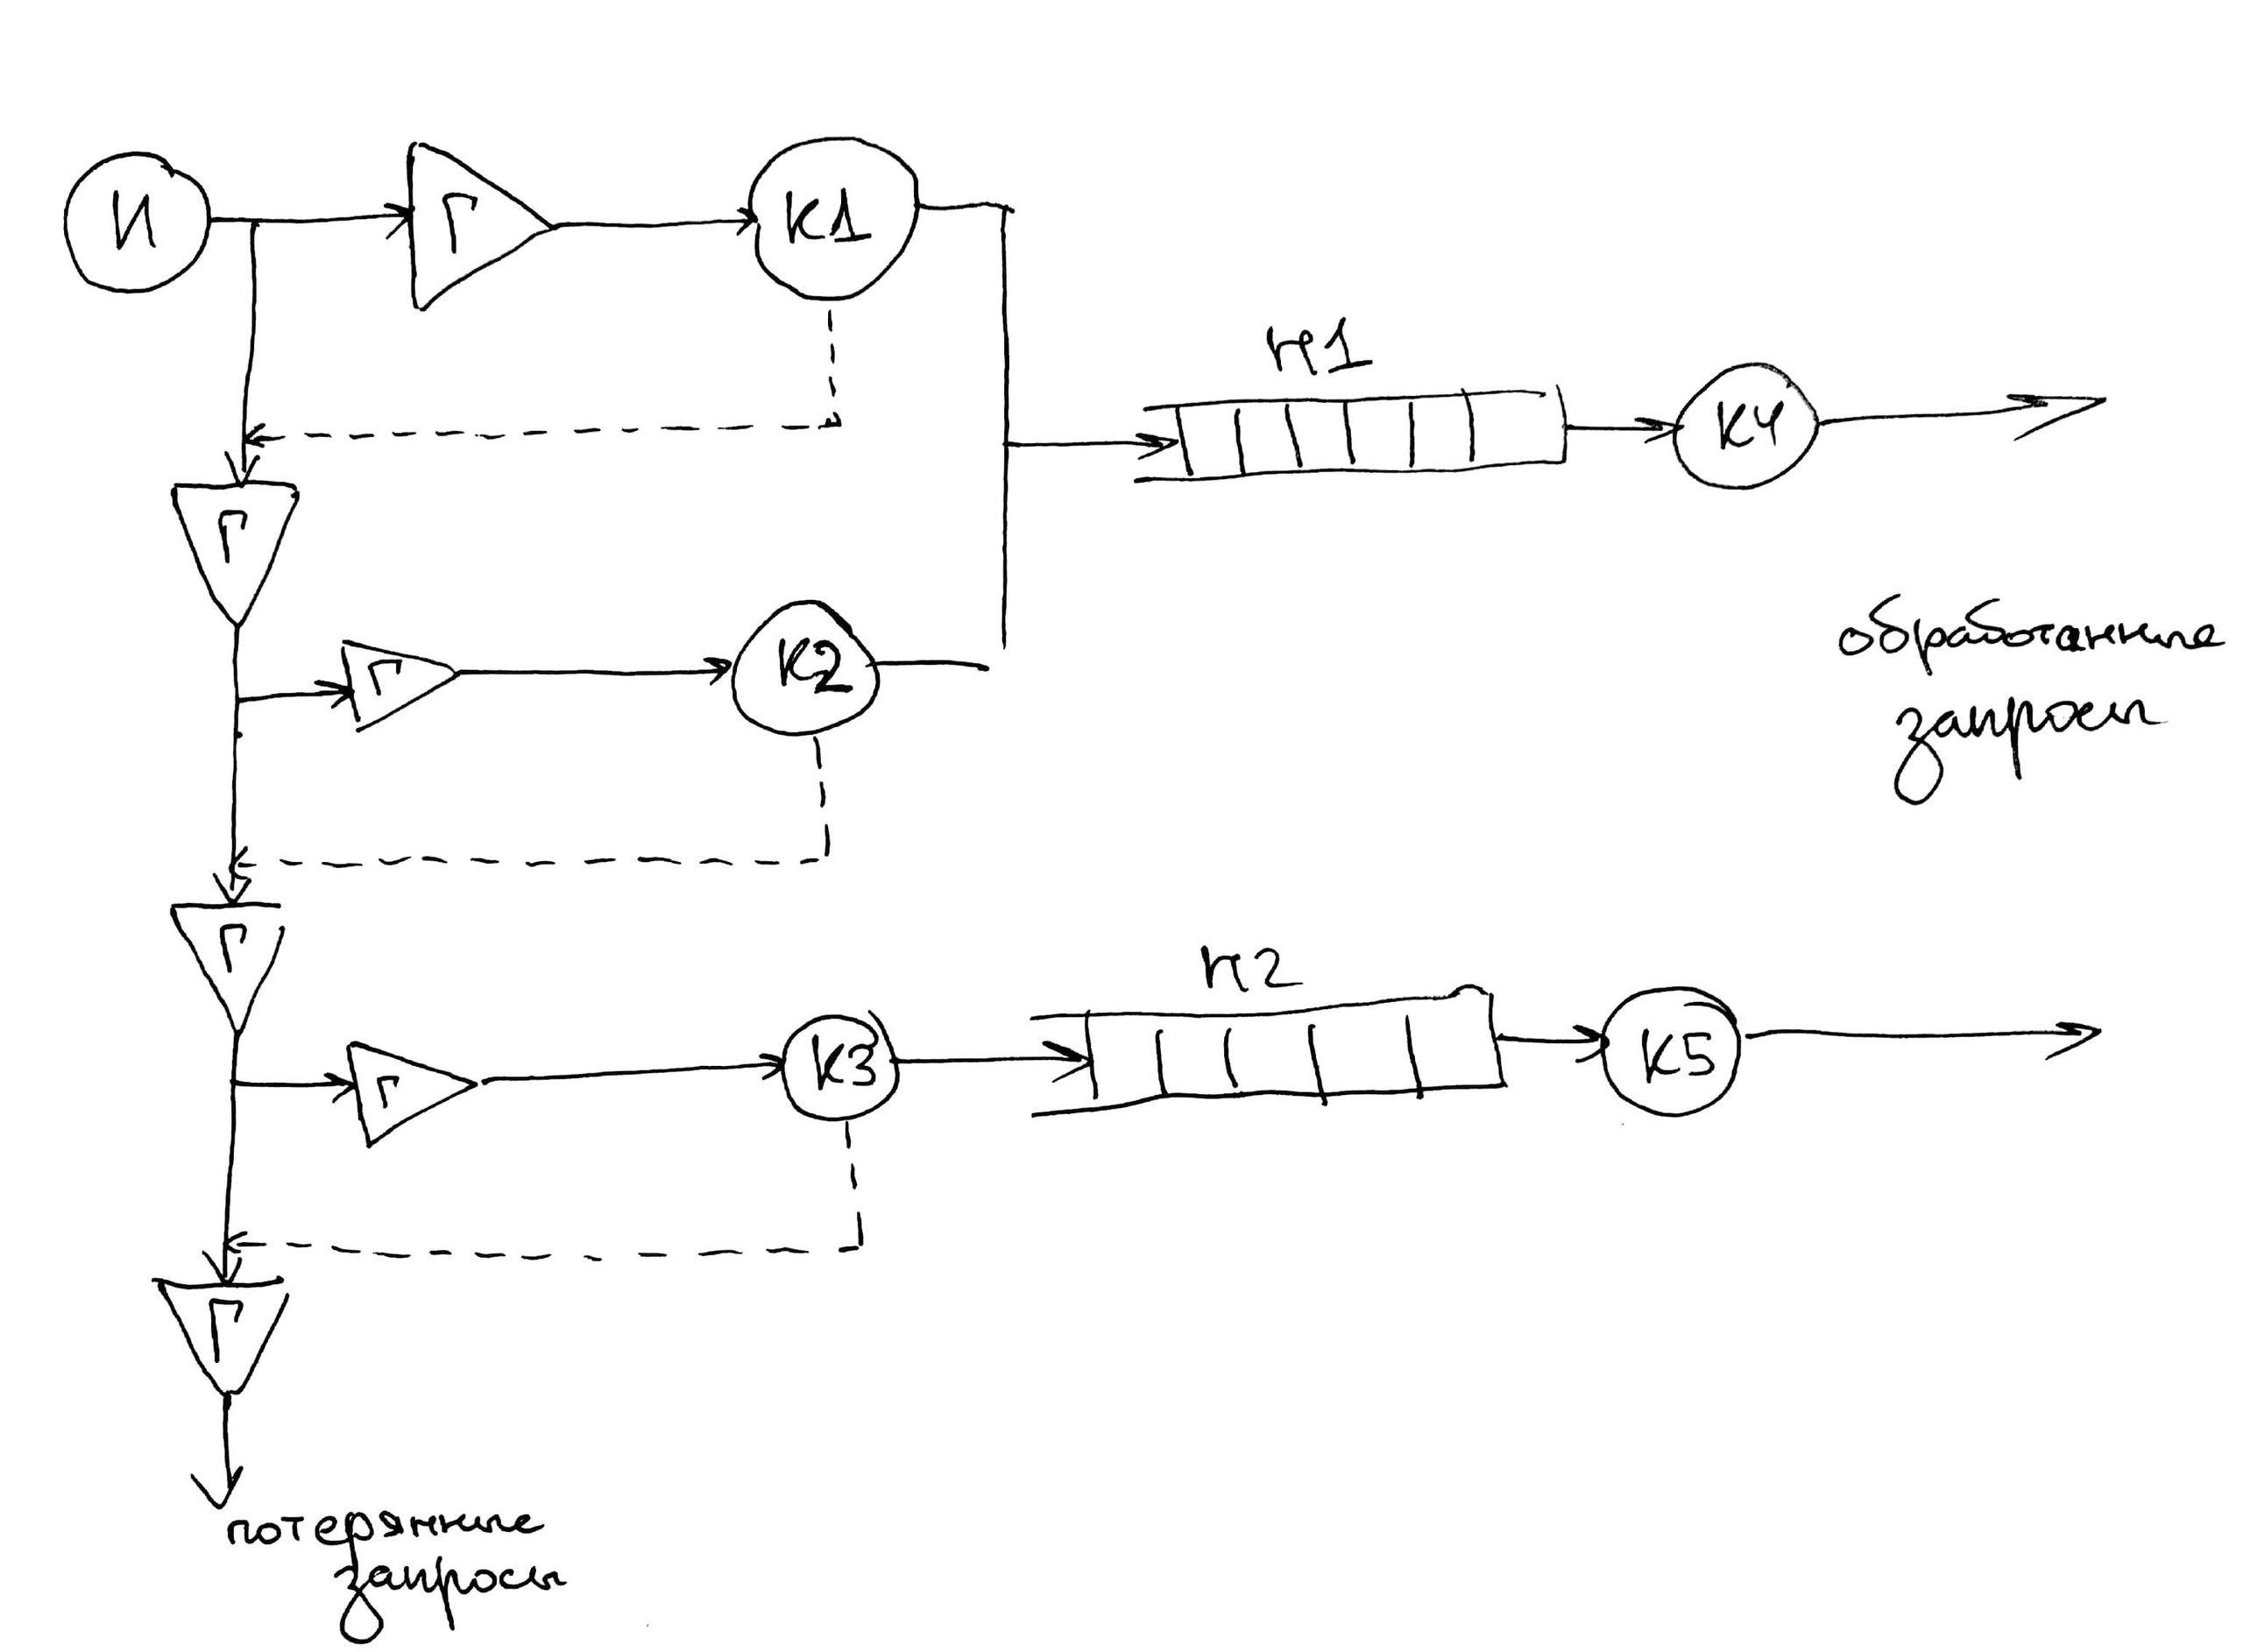
\includegraphics[width=0.9\linewidth]{inc/img/conceptual-model-qt.jpg}
	\caption{Концептуальная модель}
	\label{conceptual-model-qt}
\end{figure}

В процессе взаимодействия клиентов с информационным центром возможно:
\begin{itemize}
	\item Режим нормального обслуживания, т.е. клиент выбирает одного из свободных операторов, отдавая предпочтение тому у которого меньше номер.
	\item Режим отказа в обслуживании клиента, когда все операторы заняты.
\end{itemize}

\chapter{Листинг}

\lstinputlisting[language=GPSS]{inc/src/main.gpss}

\chapter{Результат работы}

\begin{figure}[H]
	\centering
	
\includegraphics[width=\linewidth]{inc/img/result-values.jpg}
	\caption{Сохраняемые величины]}
\end{figure}

\begin{figure}[H]
	\centering
	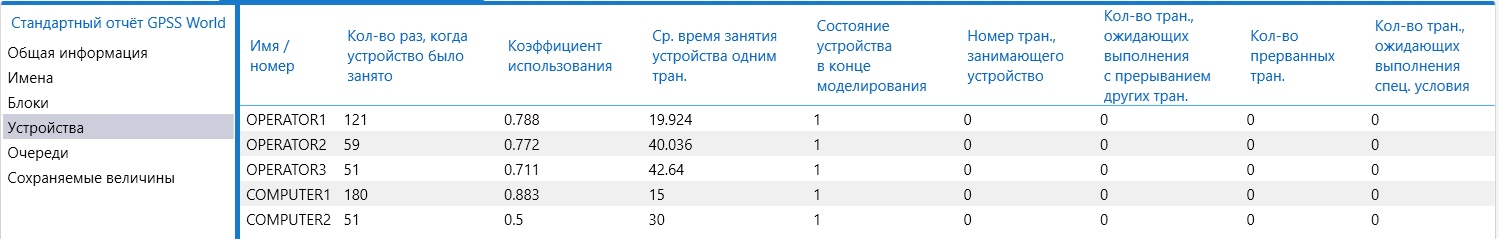
\includegraphics[width=\linewidth]{inc/img/result-devices.jpg}
	\caption{Устройства}
\end{figure}

\begin{figure}[H]
	\centering
	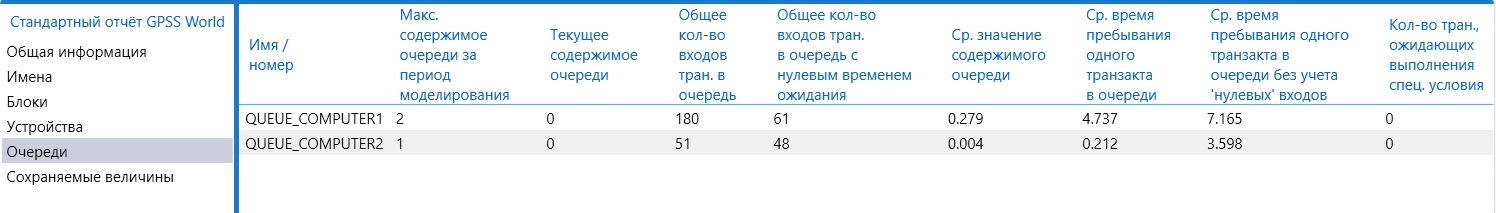
\includegraphics[width=\linewidth]{inc/img/result-queues.jpg}
	\caption{Очереди}
\end{figure}

\chapter*{Вывод}
\addcontentsline{toc}{chapter}{Вывод}

Разработана программа в системе GPSS, предназначенная для моделирования процесса обработки запросов в информационном центре, позволяющая определить количество потерянных заявок и вероятность отказа в обслуживании.

\end{document}
